Сравним точность интегрирования методом трапеций и численного интегрирования при помощи квадратуры Гаусса на примере вычисления сейсмограммы нулевого удаления отражённой волны от горизонтальной границы на глубине $H$.
Для вычисления отражённого волнового поля воспользуемся выражением \eqref{eq:modapx}. Так как вычисляется сейсмограмма нулевого удаления, то положение источника и приёмника сейсмических колебаний совпадают: $r' = r_0$. Тогда формулу  \eqref{eq:modapx} можно упростить:
\begin{equation}
			P(r_0,t') = \iint\limits_{B} \left[\Lambda(r) \frac{f'\left(t'-\frac{2|r-r_0|}{c}\right) }{16\pi^2c|r-r_0|^2} (2\cos \psi_1 ) \right] \,dB
\end{equation}
Параметризуем подынтегральное выражение с помощью $\rho = |r-r_0|$ и перейдём к полярной системе координат:
\begin{equation}
	P(r_0,t') = \int_0^{2\pi}  \int_H^{\infty} \left[\Lambda(r) \frac{f'\left(t'-\frac{2\rho}{c}\right) }{16\pi^2c\rho^2} (2\cos \psi_1 ) \right] d\rho\,d\theta.
\end{equation}
Отражающая плоскость является бесконечной, поэтому значение отражённого поля не зависит от положения источника и приёмника $r_0$ на поверхности $z=0$.
Так как плоскость горизонтальная, то $\cos \psi_1 = \frac{H}{\rho}$:
\begin{equation}
	P(t') = H \int_H^{\infty} \left[ \frac{c_2 \rho_2 \cos \theta - c_1 \rho_1 \cos \theta_2}{c_2 \rho_2 \cos \theta + c_1 \rho_1 \cos \theta_2}  \cdot \frac{f'\left(t'-\frac{2\rho}{c}\right) }{4\pi c\rho^3}  \right] d\rho,
\end{equation}
где $\cos \theta = \frac{H}{\rho}$,  $\cos \theta_2 = \sqrt{1-\frac{c_2^2 H^2}{c_1^2\rho^2}}$.

\begin{figure}[H]
	\centering
	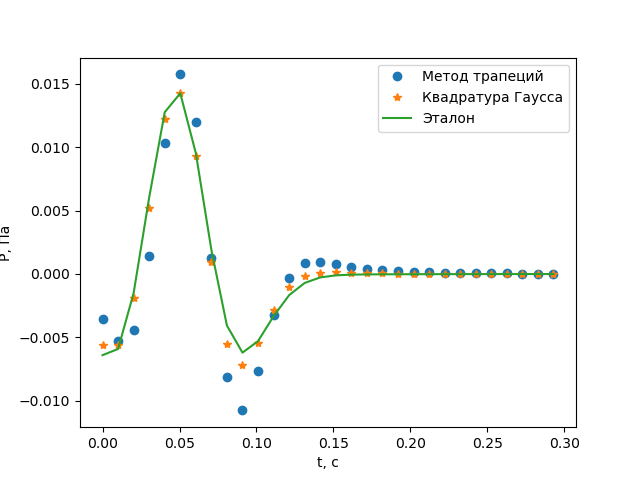
\includegraphics[width=.8\textwidth]{trapgauss.png}
	\caption{}
	\label{fig:trapgauss}
\end{figure}

На рисунке \ref{fig:trapgauss} изображены графики отражённого поля давления на поверхности, смоделированных с применением различных методов интегрирования. За эталон принимаются данные, использованные в академическом турнире.  Максимальная абсолютная погрешность вычислений с  использованием метода трапеций составляет $\Delta = 0.0046$ Па.
Максимальная абсолютная погрешность вычислений с  использованием квадратуры  Гаусса составляет $\Delta = 0.0014$ Па.
Максимальная относительная погрешность вычислений с  использованием метода трапеций составляет $\delta = 32.4\%$ .
Максимальная относительная погрешность вычислений с  использованием квадратуры  Гаусса составляет $\delta = 10\%$.

